\subsection{}
(1)下図のような頂点のラベル付けにより同型になることが確かめられる。
\begin{figure}[htbp]
  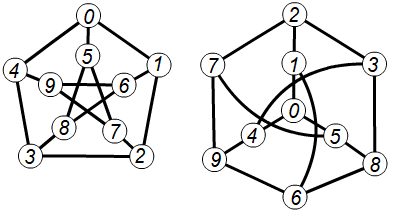
\includegraphics{chap1/fig1A1.png}
\end{figure}

(2)頂点集合を $\{1,2,3,4,5\}$の2元部分集合全体、辺集合を$\{(u,v) \mid u\cap v = \emptyset\}$ とするグラフ $G$ は注目しているグラフと同型である。
$G$ の自己同型群 $A$ は部分群として明らかに $S_5$ をもつ。
$A$ が $S_5$ と同型であることを示すために、$A$ の位数が120以下であることを示す。
固定化部分群を考えると、$A_{(1,2)}$ は $A$ の指数10の部分群である。
また$\Gamma((1,2))=\{(3,4),(3,5),(4,5)\}$であることから、$A_{(1,2),(3,4),(3,5),(4,5)}$ は $A_{(1,2)}$ の指数高々6の部分群である。
$A_{(1,2),(3,4),(3,5),(4,5)}$の位数は2であることが確かめられるので、$A$ の位数は高々 $10\times 6\times 2 =120$ である。
以上より示せた。
